%% frontmatter/titlepage.tex
%% Cover: one simulation, four views, a dashed path walking the reader
%% through the report's pipeline (noise bulk -> spikes detach -> the
%% eigenvector lights up -> the embedding clusters). The background artwork
%% (figures/titlepage_background.pdf) is generated by
%% notebooks/06_titlepage_art.py; the type is overlaid via TikZ in the
%% artwork's clear zones: the title at the top, the author block in the
%% void beside panel 4.

\thispagestyle{empty}

\definecolor{coverInk}{HTML}{2D2D2D}
\definecolor{coverSlate}{HTML}{3A5A78}
\definecolor{coverGray}{HTML}{8B8378}

\begin{tikzpicture}[remember picture, overlay]
  % full-bleed background artwork
  \node[anchor=center, inner sep=0pt] at (current page.center)
    {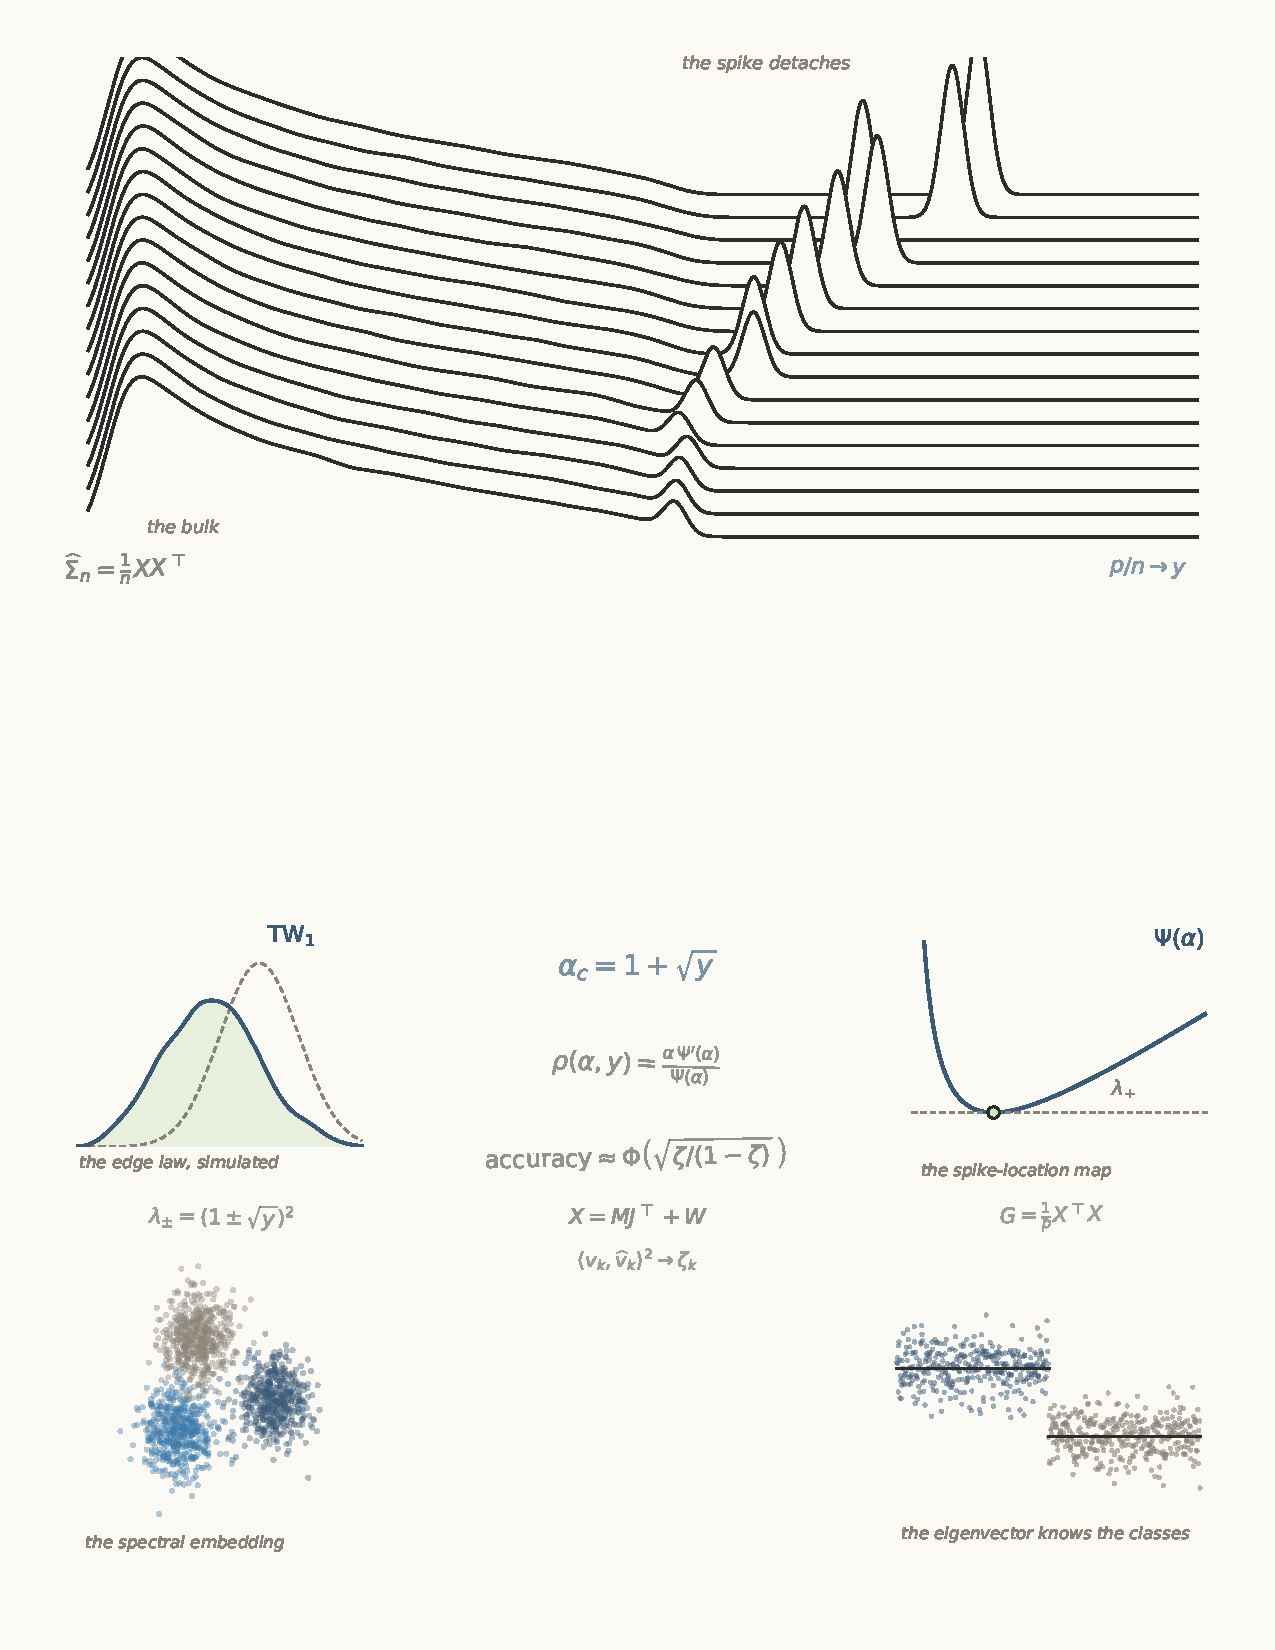
\includegraphics[width=\paperwidth, height=\paperheight]{figures/titlepage_background.pdf}};

  % ----- title, big, at the top, above the story
  \node[anchor=center] at ([yshift=-0.95in]current page.north)
    {\fontsize{24}{29}\selectfont\bfseries\textcolor{coverInk}{A STUDY OF RANDOM MATRICES}};

  \node[anchor=center] at ([yshift=-1.42in]current page.north)
    {\fontsize{13.5}{17}\selectfont\itshape\textcolor{coverSlate}{From Foundations to Spectral Clustering}};

  % ----- author block, in the void beside panel 4
  \node[anchor=center] at ([xshift=-2.04in, yshift=2.46in]current page.south)
    {\large\textcolor{coverInk}{ARZAAN SINGH}};

  \node[anchor=center] at ([xshift=-2.04in, yshift=2.18in]current page.south)
    {\footnotesize\textcolor{coverInk}{Under the supervision of Professor Gustavo Didier}};

  \node[anchor=center] at ([xshift=-2.04in, yshift=1.92in]current page.south)
    {\footnotesize\itshape\textcolor{coverGray}{An Independent Study Report}};

  \node[anchor=center] at ([xshift=-2.04in, yshift=1.66in]current page.south)
    {\footnotesize\textcolor{coverInk}{Department of Mathematics \,\(\cdot\)\, Tulane University}};

  \node[anchor=center] at ([xshift=-2.04in, yshift=1.40in]current page.south)
    {\footnotesize\textcolor{coverInk}{June 2026}};

  % ----- one-line colophon at the foot
  \node[anchor=south] at ([yshift=0.30in]current page.south)
    {\fontsize{7}{9}\selectfont\textcolor{coverGray}{%
      Cover: one simulated data set, read four ways, exactly as in the report; generated by \texttt{notebooks/06\_titlepage\_art.py}.}};
\end{tikzpicture}

\clearpage
